\documentclass[a4paper, 12pt]{report}
\usepackage{color, xcolor} % 使用颜色
\usepackage[utf8]{inputenc} % 使用utf8编码
\usepackage{hyperref} % 使用\href, \url
\usepackage{enumitem} % 使用\enumerate
\usepackage{float} % 使用[H]标签,让图片和文字一起浮动
\usepackage{caption} % 使用\caption*
\usepackage{amsmath}
\usepackage{mathrsfs, bm, amsfonts, amssymb, bbm}
\usepackage{graphicx}
\graphicspath{{../img/}}
\usepackage{geometry}
\geometry{left=3cm, right=2.5cm, top=2.5cm, bottom=2.5cm}

\usepackage{listings}
\lstset{
  basicstyle=\ttfamily,
  columns=fullflexible,
  breaklines=true,
}

\usepackage[most]{tcolorbox}
\newtcblisting{commandshell}{colback=white,colupper=black,colframe=black!75!black,
listing only,listing options={language=sh, breaklines=true,aboveskip=0pt, belowskip=0pt},
every listing line={\small\ttfamily\bfseries{[shchai@alan]\$} }}

\title{Security Models Experiment Report}
\date{}
\author{Shitong CHAI}

\begin{document}

\maketitle
\tableofcontents

\chapter* {Exercise 1(AVISPA)}
\addcontentsline{toc}{chapter}{\protect\numberline{}Exercise 1}%
    \section*{1. OFMC, Cl-Atse, SATMC, TA4SP}
    Firstly, using web interface to analyse NSPK. I can use 4 different tools to analyse NSPK, the configuration of OFMC is shown in Figure \ref{avispaweb}.
    \begin{figure}[H]
        \centering
        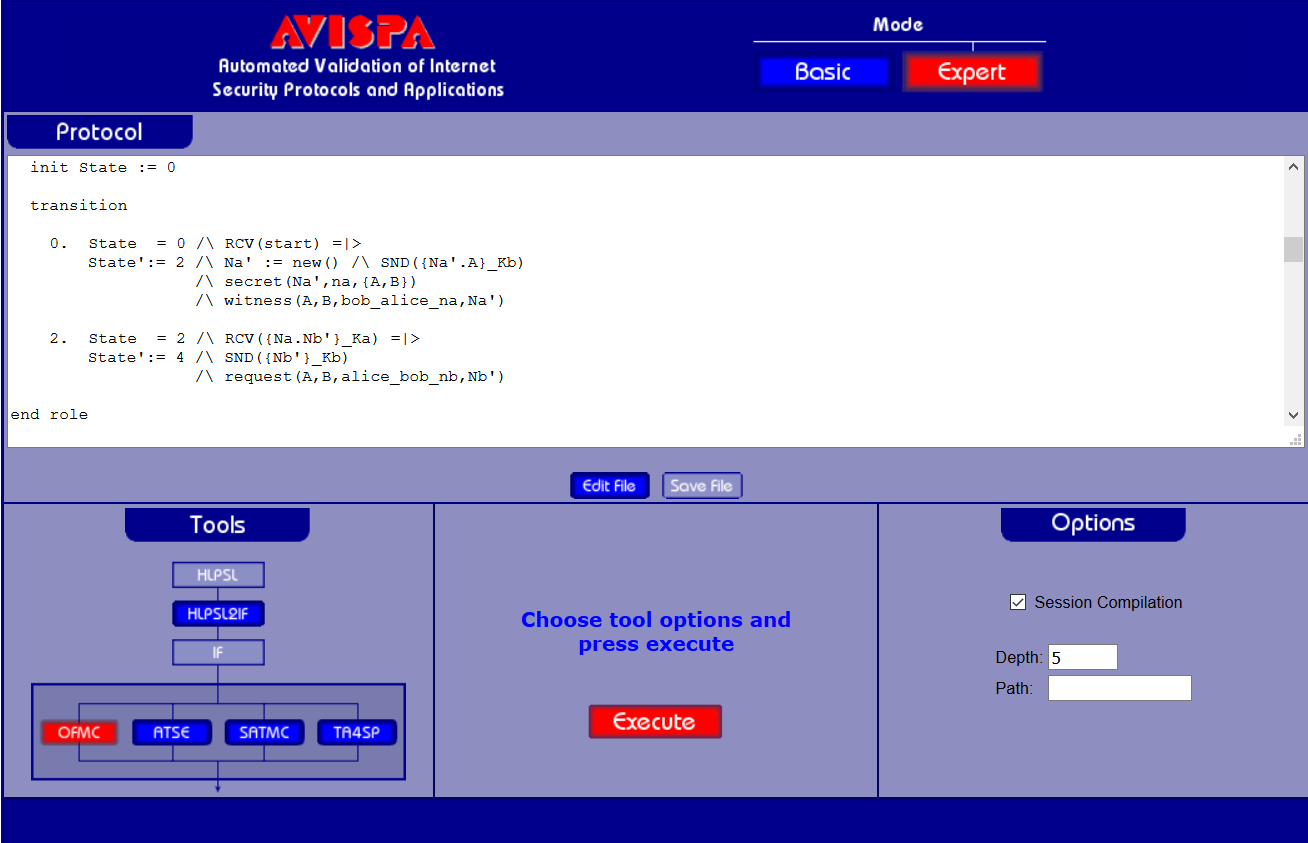
\includegraphics[width=0.8\textwidth]{avispaweb}
        \caption{Avispa web interface for NSPK analysis with OFMC}
        \label{avispaweb}
    \end{figure}

    The execution always fails with the following page:

    \begin{figure}[H]
        \centering
        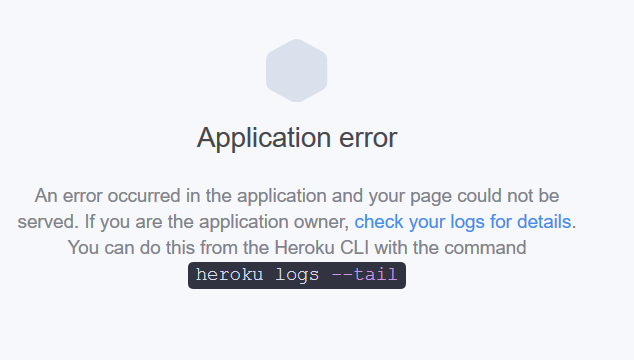
\includegraphics[width=0.5\textwidth]{errorpage}
        \caption{Avispa web interface error page}
        \label{errorpage}
    \end{figure}

    Secondly, using command line to analyse NSPK.
        \begin{commandshell}
avispa NSPK.hlpsl --ofmc > NSPK.ofmc
avispa NSPK.hlpsl --cl-atse > NSPK.cl-atse
avispa NSPK.hlpsl --satmc > NSPK.satmc
avispa NSPK.hlpsl --ta4sp > NSPK.ta4sp
        \end{commandshell}
        The content of output files are as listed below.

        The file \emph{NSPK.ofmc} is as follows.
        \begin{lstlisting}[frame=single]
% OFMC
% Version of 2006/02/13
SUMMARY
  UNSAFE
DETAILS
  ATTACK_FOUND
PROTOCOL
  /home/local.isima.fr/shchai/.avispa/results/NSPK.if
GOAL
  secrecy_of_nb
BACKEND
  OFMC
COMMENTS
STATISTICS
  parseTime: 0.00s
  searchTime: 0.01s
  visitedNodes: 10 nodes
  depth: 2 plies
ATTACK TRACE
i -> (a,6): start
(a,6) -> i: {Na(1).a}_ki
i -> (b,3): {Na(1).a}_kb
(b,3) -> i: {Na(1).Nb(2)}_ka
i -> (a,6): {Na(1).Nb(2)}_ka
(a,6) -> i: {Nb(2)}_ki
i -> (i,17): Nb(2)
i -> (i,17): Nb(2)


% Reached State:
% 
% secret(Nb(2),nb,set_70)
% witness(b,a,alice_bob_nb,Nb(2))
% contains(a,set_70)
% contains(b,set_70)
% secret(Na(1),na,set_74)
% witness(a,i,bob_alice_na,Na(1))
% contains(a,set_74)
% contains(i,set_74)
% state_bob(b,i,ki,kb,1,dummy_nonce,dummy_nonce,set_78,10)
% state_alice(a,i,ka,ki,4,Na(1),Nb(2),set_74,6)
% state_bob(b,a,ka,kb,3,Na(1),Nb(2),set_70,3)
% state_alice(a,b,ka,kb,0,dummy_nonce,dummy_nonce,set_62,3)
% request(a,i,alice_bob_nb,Nb(2),6)
        \end{lstlisting}
        The file \emph{NSPK.cl-atse} is as follows.
        \begin{lstlisting}[frame=single]

SUMMARY
  UNSAFE

DETAILS
  ATTACK_FOUND
  TYPED_MODEL

PROTOCOL
  /home/local.isima.fr/shchai/.avispa/results/NSPK.if

GOAL
  Secrecy attack on (n5(Nb))

BACKEND
  CL-AtSe

STATISTICS

  Analysed   : 9 states
  Reachable  : 8 states
  Translation: 0.00 seconds
  Computation: 0.00 seconds


ATTACK TRACE
 i -> (a,6):  start
 (a,6) -> i:  {n9(Na).a}_ki
              & Secret(n9(Na),set_74);  Add a to set_74;  Add i to set_74;

 i -> (a,3):  start
 (a,3) -> i:  {n1(Na).a}_kb
              & Secret(n1(Na),set_62);  Witness(a,b,bob_alice_na,n1(Na));
              & Add a to set_62;  Add b to set_62;

 i -> (b,4):  {n9(Na).a}_kb
 (b,4) -> i:  {n9(Na).n5(Nb)}_ka
              & Secret(n5(Nb),set_70);  Witness(b,a,alice_bob_nb,n5(Nb));
              & Add a to set_70;  Add b to set_70;

 i -> (a,6):  {n9(Na).n5(Nb)}_ka
 (a,6) -> i:  {n5(Nb)}_ki

        \end{lstlisting}
        The file \emph{NSPK.satmc} is as follows.
        \begin{lstlisting}[frame=single]
SUMMARY
  UNSAFE

DETAILS
  ATTACK_FOUND
  BOUNDED_NUMBER_OF_SESSIONS
  BOUNDED_SEARCH_DEPTH
  BOUNDED_MESSAGE_DEPTH

PROTOCOL
  NSPK.if

GOAL
  secrecy_of_nb(nb0(b,4),set_70)

BACKEND
  SATMC

COMMENTS

STATISTICS
  attackFound               true      boolean
  upperBoundReached         false     boolean
  graphLeveledOff           no        boolean
  satSolver                 sim       solver
  maxStepsNumber            30        steps
  stepsNumber               5         steps
  atomsNumber               379       atoms
  clausesNumber             993       clauses
  encodingTime              0.05      seconds
  solvingTime               0.0       seconds
  if2sateCompilationTime    0.01      seconds

ATTACK TRACE
  i       ->    (a,6)    : start
  (a,6)   ->    i        : {na0(a,6).a}_ki
  i       ->    (b,4)    : {na0(a,6).a}_kb
  (b,4)   ->    i        : {na0(a,6).nb0(b,4)}_ka
  i       ->    (a,6)    : {na0(a,6).nb0(b,4)}_ka
  (a,6)   ->    i        : {nb0(b,4)}_ki
        \end{lstlisting}
        The file \emph{NSPK.ta4sp} is as follows.
        \begin{lstlisting}[frame=single]
SUMMARY
   INCONCLUSIVE

DETAILS
   OVER_APPROXIMATION
   UNBOUNDED_NUMBER_OF_SESSIONS
   TYPED_MODEL

PROTOCOL
   /home/local.isima.fr/shchai/.avispa/results/NSPK.if.ta4sp

GOAL
   SECRECY - Property with identitier: nb

BACKEND
   TA4SP

COMMENTS
   Use an under-approximation in order to show a potential attack
   The intruder might know some critical information
 

STATISTICS
   Translation: 0.00 seconds
   Computation 0.40 seconds


ATTACK TRACE
   No Trace can be provided with the current version.
        \end{lstlisting}

    \section*{2. Understand the results}

        For OFMC(file \emph{NSPK.ofmc}), the summary is \emph{unsafe}, which is correct about NSPK. The attack will focus on the secret which is identified with the constant \emph{nb}, which means the variable \emph{Nb'} sent by bob is not a secret of agent set \{A, B \} anymore, where A plays role alice and B plays role bob. The attack trace is a standard \emph{man-in-the-middle} attack. Intruder i sends \emph{start} to a, a sends back \emph{Na} and \emph{a} back, then
        \emph{i} fakes sender \emph{a}, and sends \emph{Na} and \emph{a} encrypted with \emph{kb} to \emph{b}. \emph{b} thinks the sender is \emph{a} and sends the target \emph{Nb} encrypted with \emph{ka} back. In the end, \emph{i} uses \emph{a} to decrypt the target \emph{Nb}. So the secret \emph{Nb} is compromised. The secret is lost because of lack of authentication on the sender.
            
        For Cl-Atse(file \emph{NSPK.cl-atse}), the attack is also on \emph{Nb}. Intruder \emph{i} sends \emph{start} to \emph{a} and \emph{a} sends back \emph{Na} and \emph{a}. Then \emph{i} fakes \emph{b} and send start to \emph{a} and \emph{a} sends \emph{Na} and \emph{a} encrypted with \emph{kb} to \emph{i}, which is then sent to \emph{b}. \emph{b} sends back to \emph{i} the target \emph{Nb} encrypted with \emph{ka} which is decrypted by utilizing \emph{a}.
            
        For SATMC(file \emph{NSPK.satmc}), the attack is also on \emph{Nb}. The attack trace is exactly the same as OFMC.
            
        For TA4SP(file \emph{NSPK.ta4sp}), the summary is inconclusive and no attack trace was found.

    \section*{3. Correction}
        The corrected source file \emph{NSPK-fix.hlpsl} is as follows:
        \begin{lstlisting}[frame=single]
%% PROTOCOL: NSPK: Needham-Schroeder Public-Key Protocol
%% VARIANT: original version (of 1978) without key server
%% PURPOSE: Two-party mutual autentication
%% MODELER: David von Oheimb, Siemens CT IC 3, January 2005
%% ALICE_BOB:
%%\begin{verbatim}
%% 1. A  - {Na.A}_Kb ----> B
%% 2. A  B
%%\end{verbatim}
%% PROBLEMS: 3
%% CLASSIFICATION: G1, G3, G12
%% ATTACKS: Man-in-the-middle attack,
%% where in the first session Alice talks with the intruder as desired
%% and in the second session Bob wants to talk with Alice but actually
%% talks to the intruder. Therefore, also the nonce Nb gets leaked.
%%\begin{verbatim}
%% 1.1  A  - {Na.A}_Ki --> i   	
%% 2.1                     i(A)  - {Na.A}_Kb  -> B   	
%% 2.2                     i(A)  B
%%\end{verbatim}
%%%%%%%%%%%%%%%%%%%%%%%%%%%%%%%%%%%%%%%%%%%%%%%%%%%%%%%%%%%%%%%%%%%%%%%%
%%HLPSL:
role alice (A, B: agent,             
            Ka, Kb: public_key,      
            SND, RCV: channel (dy)) 
played_by A def=

  local State : nat, 
        Na, Nb: text

  init State := 0

  transition  
   
    0.  State  = 0 /\ RCV(start) =|> 
	State':= 2 /\ Na' := new() /\ SND({Na'.A}_Kb)
		   /\ secret(Na',na,{A,B}) 
		   /\ witness(A,B,bob_alice_na,Na')

    2.  State  = 2 /\ RCV({Na.Nb'.B}_Ka) =|> 
	State':= 4 /\ SND({Nb'}_Kb) 
		   /\ request(A,B,alice_bob_nb,Nb')

end role

%%%%%%%%%%%%%%%%%%%%%%%%%%%%%%%%%%%%%%%%%%%%%%%%%%%%%%%%%%%%%%%%%%%%%%%%

role bob(A, B: agent,      
         Ka, Kb: public_key,      
         SND, RCV: channel (dy)) 
played_by B def=

  local State : nat, 
	Na, Nb: text

  init State := 1

  transition 

    1.  State  = 1 /\ RCV({Na'.A}_Kb) =|> 
	State':= 3 /\ Nb' := new() /\ SND({Na'.Nb'.B}_Ka)
		   /\ secret(Nb',nb,{A,B})  % nb is the name of this secret
		   /\ witness(B,A,alice_bob_nb,Nb')

    3.  State  = 3 /\ RCV({Nb}_Kb) =|> 
	State':= 5 /\ request(B,A,bob_alice_na,Na)

end role

%%%%%%%%%%%%%%%%%%%%%%%%%%%%%%%%%%%%%%%%%%%%%%%%%%%%%%%%%%%%%%%%%%%%%%%%

role session(A, B: agent, Ka, Kb: public_key) def=

  local SA, RA, SB, RB: channel (dy)

  composition 

	alice(A,B,Ka,Kb,SA,RA)
     /\ bob  (A,B,Ka,Kb,SB,RB)

end role

%%%%%%%%%%%%%%%%%%%%%%%%%%%%%%%%%%%%%%%%%%%%%%%%%%%%%%%%%%%%%%%%%%%%%%%%

role environment() def=

    const a, b	       : agent,
	  ka, kb, ki   : public_key,
	  na, nb,
	  alice_bob_nb,
	  bob_alice_na : protocol_id

    intruder_knowledge = {a, b, ka, kb, ki, inv(ki)}

    composition

	session(a,b,ka,kb)
     /\ session(a,i,ka,ki)
     /\ session(i,b,ki,kb)

end role

%%%%%%%%%%%%%%%%%%%%%%%%%%%%%%%%%%%%%%%%%%%%%%%%%%%%%%%%%%%%%%%%%%%%%%%%

goal

  secrecy_of na, nb
  authentication_on alice_bob_nb
  authentication_on bob_alice_na

end goal

%%%%%%%%%%%%%%%%%%%%%%%%%%%%%%%%%%%%%%%%%%%%%%%%%%%%%%%%%%%%%%%%%%%%%%%%

environment()
        \end{lstlisting}
    \section*{4. Compare with \emph{NSPK-fix-Lowe.hlspl}}
    The code is exactly the same, both adding identification constant \emph{B} in the message encrypted by \emph{a} and sent to \emph{b}.
            
\chapter* {Exercise 2(SCYTHER)}
\addcontentsline{toc}{chapter}{\protect\numberline{}Exercise 2}%
    \section*{a. Why is the property violated?}
    For the claim that \emph{ni} is a secret for \emph{I}, it's violated because an attacker \emph{Eve} can intercept the message from \emph{Bob} to \emph{Alice}, namely \emph{\{Alice, ni\}} to fake and replay as \emph{Alice} and get the target \emph{ni} encrypted with his public key \emph{pk(Eve)}. This attack is because of lack of authentication on the session initializer. The attack trace is shown in Figure \ref{i1ni}.
    \begin{figure}[H]
        \centering
        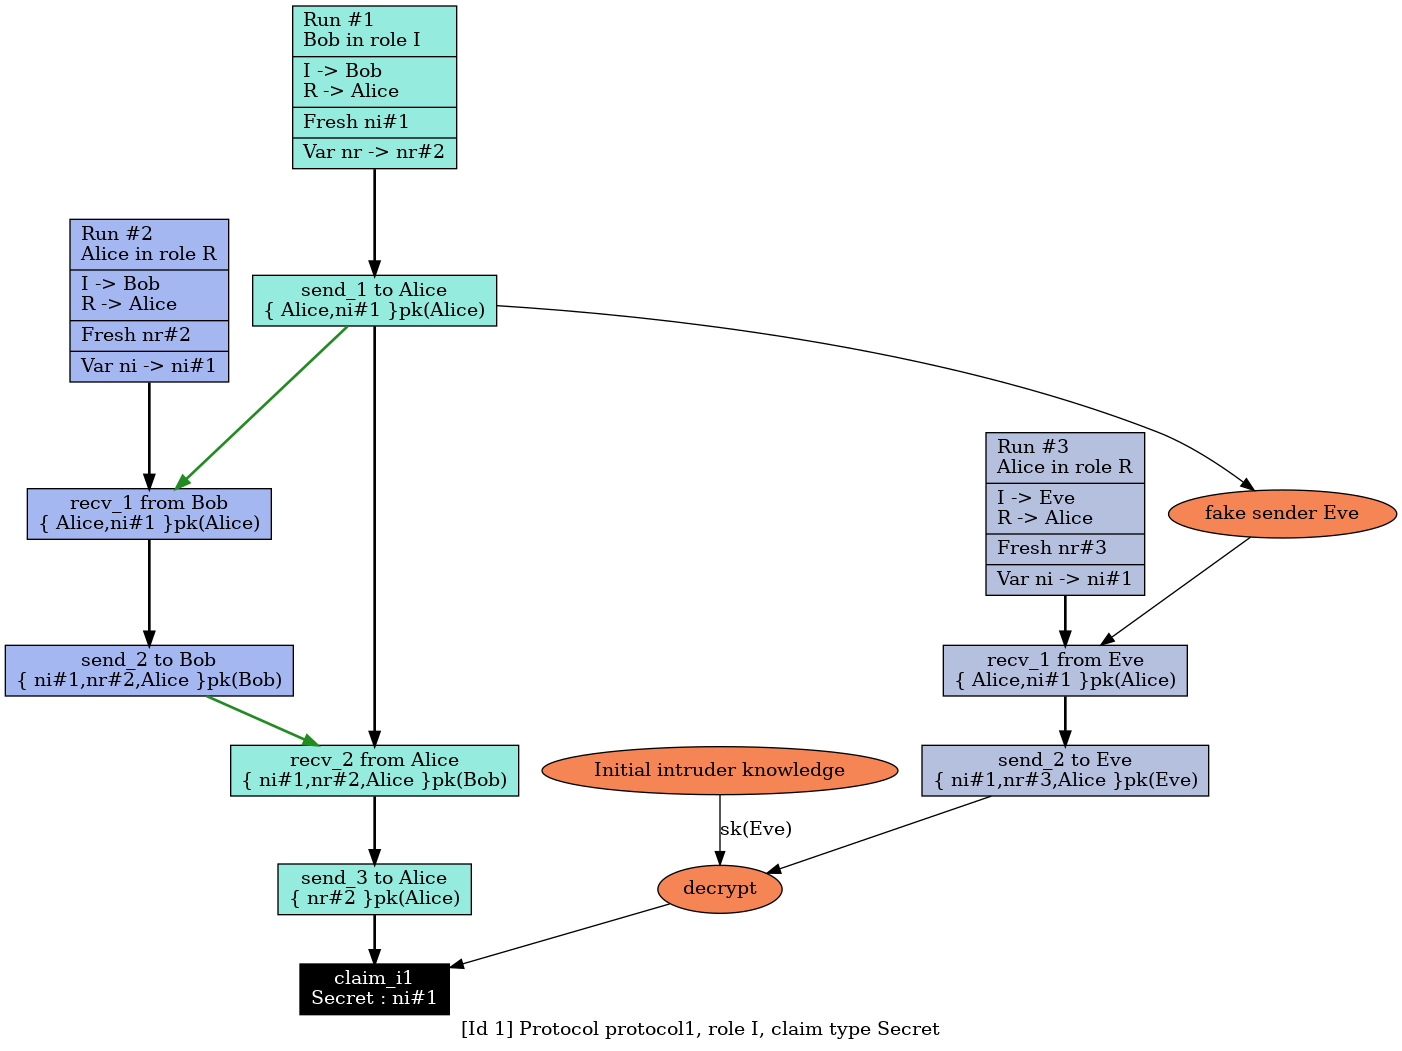
\includegraphics[width=0.8\textwidth]{i1ni}
        \caption{Attack trace for \emph{I}'s secret \emph{ni}}
        \label{i1ni}
    \end{figure}
    For the claim that \emph{nr} is a secret for \emph{I}, it's violated because the attacker can fake \emph{Bob} and get the target encrypted with his public key, then he replace the \emph{nr} with his nonce. The attack trace is shown in Figure \ref{i2nr}.
    \begin{figure}[H]
        \centering
        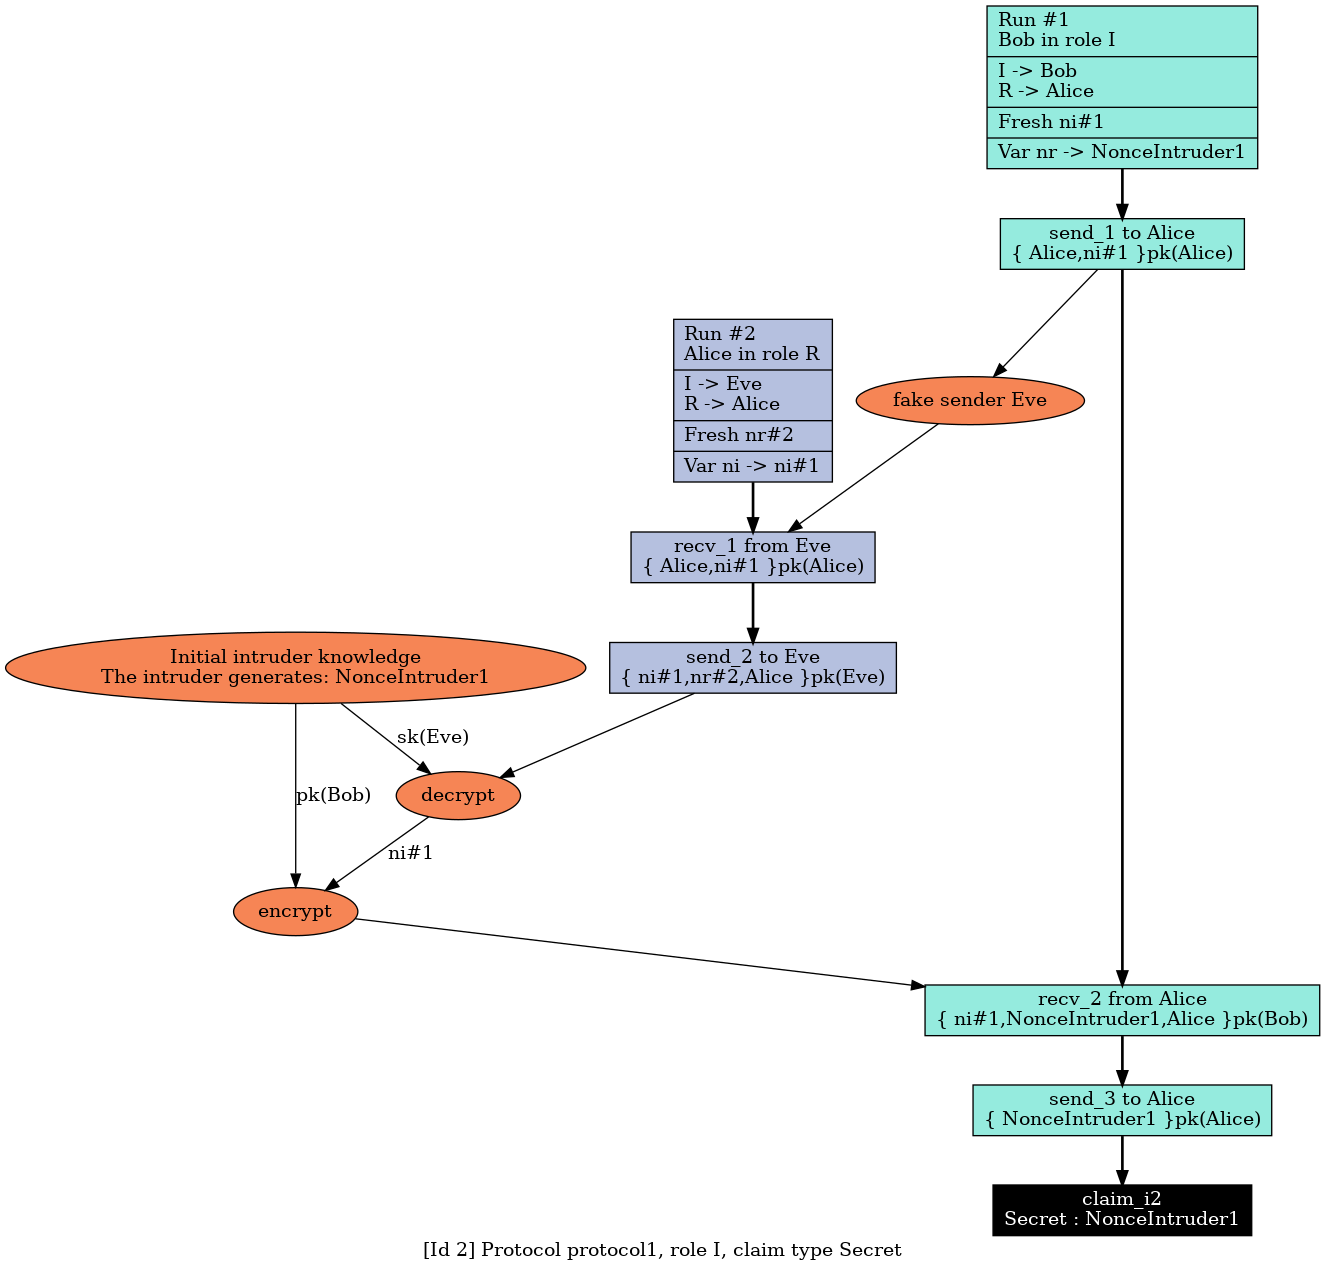
\includegraphics[width=0.8\textwidth]{i2nr}
        \caption{Attack trace for \emph{I}'s secret \emph{nr}}
        \label{i2nr}
    \end{figure}
    For the claim that nonce is synchronized between \emph{I} and \emph{R}. It is violated because of the same reason as the last claim, the message \emph{ni} is replaced with the nonce of intruder, so it is not synchronized. The attack trace exactly the same as \ref{i2nr}.
    \section*{b. Correction}
        The corrected file \emph{protocol1fixed.spdl} is shown below.
        \begin{lstlisting}[frame=single]
/* 
 * Fixed protocol
 */

// PKI infrastructure

const pk: Function;
secret sk: Function;
inversekeys (pk,sk);

// The protocol description

protocol protocol1(I,R)
{
	role I
	{
		const ni: Nonce;
		var nr: Nonce;

		send_1(I,R, {R,ni,I}pk(R) );
		read_2(R,I, {ni,nr,R}pk(I) );
		send_3(I,R, {nr}pk(R) );

		claim_i1(I,Secret,ni);
		claim_i2(I,Secret,nr);
		claim_i3(I,Nisynch);
	}

	role R
	{
		var ni: Nonce;
		const nr: Nonce;

		read_1(I,R, {R,ni,I}pk(R) ); // add identification I
		send_2(R,I, {ni,nr,R}pk(I) );
		read_3(I,R, {nr}pk(R) );

		claim_r1(R,Secret,ni);
		claim_r2(R,Secret,nr);
		claim_r3(R,Nisynch);
	}
}

// An untrusted agent, with leaked information

const Eve: Agent;
untrusted Eve;
compromised sk(Eve);
        \end{lstlisting}
        The protocol is fixed in the same way as NSPK, just adding identification constant in the encrypted message sent to receiver will keep the receiver from \emph{man-in-the-middle} attack. The checking result is shown in Figure \ref{fixedp1}.
    \begin{figure}[H]
        \centering
        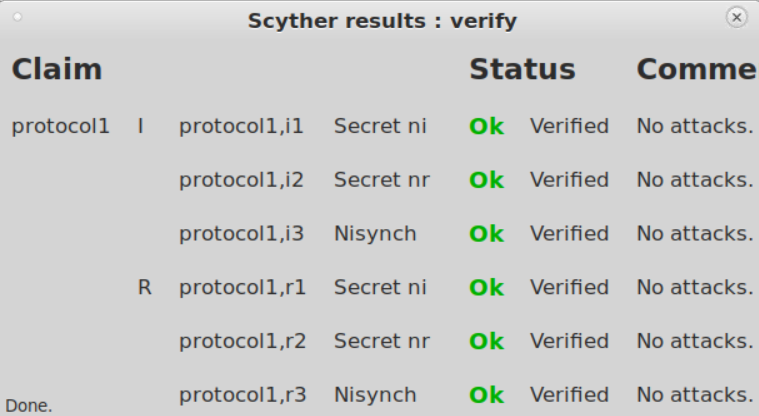
\includegraphics[width=0.8\textwidth]{fixedp1}
        \caption{Checking result of the fixed protocol}
        \label{fixedp1}
    \end{figure}
\chapter* {Exercise 3(SCYTHER)}
\addcontentsline{toc}{chapter}{\protect\numberline{}Exercise 3}%
    \section*{Improvement}
    \begin{enumerate}
        \item Remove \emph{nr}.

            Sending \emph{nr} is redundant and doesn't help in exchanging \emph{kir} safely.
        \item Add hash computation for \emph{ni} and \emph{I} in the first message.

            The size of message can be reduced by introducing hash computation for \emph{ni} and \emph{I} since hash function is one-way, the hashed value is enough for authentication.
        \item Remove \emph{kir} from hash function.

            \emph{kir} is the key to exchange and is already in the encrypted message, computing its hashed value is redundant.

        \item Change the content of the third message to \emph{I}.

            Actually, the content of the third message can be any constant as long as it is encrypted by \emph{kir}, so I take the identification constant of \emph{I}.
        \item Add hash computation for the third message.

            The size of message can be reduced by introducing hash computation since hash function is one-way, the hashed value is enough for authentication.
    \end{enumerate}

    The complete code is shown below.
    \begin{lstlisting}[frame=single]
/* 
   A key exchange protocol
*/

// PKI

const pk: Function;
secret sk: Function;
inversekeys (pk,sk);

// Hash function: nobody knows the inverse

const hash: Function;
secret unhash: Function;
inversekeys (hash,unhash);

// User type declaration

usertype Key;

// Protocol description

protocol protocol2(I,R)
{
	role I
	{
		const ni: Nonce;
		var nr: Nonce;
		var kir: Key;

		send_1 (I,R, { hash(ni, I) }pk(R) );
		read_2 (R,I, { hash(ni, R),kir }pk(I) );
		send_3 (I,R, { hash(I) }kir );
		claim_i1 (I, Secret, kir );
		claim_i2 (I, Nisynch );
	}

	role R
	{
		var ni: Nonce;
		const nr: Nonce;
		const kir: Key;

		read_1 (I,R, { hash(ni, I) }pk(R) );
		send_2 (R,I, { hash(ni, R),kir }pk(I) );
		read_3 (I,R, { hash(I) }kir );
		claim_r1 (R, Secret, kir );
		claim_r2 (R, Nisynch );
	}
}

// An untrusted agent, with compromised key

const e: Agent;
untrusted e;
compromised sk(e);
    \end{lstlisting}
    The checking result is shown in Figure \ref{imp}

    \begin{figure}[H]
        \centering
        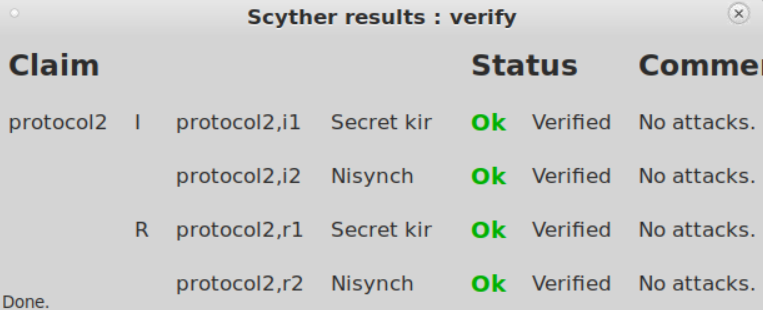
\includegraphics[width=0.8\textwidth]{imp}
        \caption{Checking result of improved protocol}
        \label{imp}
    \end{figure}
\chapter* {Exercise 4(Proverif with Horn Clauses)}
\addcontentsline{toc}{chapter}{\protect\numberline{}Exercise 4}%
    \section*{1. Check}
        I use the following command to check the file \emph{needham.horn}.
        \begin{commandshell}
proverif -in horn needham.horn > needham.proverif
        \end{commandshell}
        The checking result is stored in the file \emph{needham.proverif} which is shown below.
        \begin{lstlisting}[frame=single]
Initial clauses:
Clause 14: c:(v_25,v_26) -> c:v_26
Clause 13: c:(v_20,v_21) -> c:v_20
Clause 12: c:v_18 & c:v_19 -> c:(v_18,v_19)
Clause 11: c:c[]
Clause 10: c:pk(sA[])
Clause 9: c:pk(sB[])
Clause 8: c:x_17 & c:encrypt(m_16,pk(x_17)) -> c:m_16
Clause 7: c:x_15 -> c:pk(x_15)
Clause 6: c:x_14 & c:y_13 -> c:encrypt(x_14,y_13)
Clause 5: c:pk(x_12) -> c:encrypt((Na[pk(x_12)],pk(sA[])),pk(x_12))
Clause 4: c:pk(x_10) & c:encrypt((Na[pk(x_10)],y_11),pk(sA[])) -> c:encrypt((y_11,k[pk(x_10)]),pk(x_10))
Clause 3: c:encrypt((x_8,y_9),pk(sB[])) -> c:encrypt((x_8,Nb[x_8,y_9]),y_9)
Clause 2: c:encrypt((x_6,pk(sA[])),pk(sB[])) & c:encrypt((Nb[x_6,pk(sA[])],z_7),pk(sB[])) -> c:encrypt(secret[],pk(z_7))
Clause 1: c:new-name[!att = v_4]
Completing...
goal reachable: c:secret[]
Abbreviations:
Na_190 = Na[pk(x_174)]
Nb_191 = Nb[Na_190,pk(sA[])]
k_192 = k[pk(x_174)]
clause 8 c:secret[]
    duplicate c:x_188
    clause 2 c:encrypt(secret[],pk(x_188))
        duplicate c:encrypt((Na_190,pk(sA[])),pk(sB[]))
        clause 6 c:encrypt((Nb_191,x_188),pk(sB[]))
            apply 2-tuple c:(Nb_191,x_188)
                apply 1-proj-2-tuple c:Nb_191
                    clause 8 c:(Nb_191,k_192)
                        duplicate c:x_174
                        clause 4 c:encrypt((Nb_191,k_192),pk(x_174))
                            duplicate c:pk(x_174)
                            clause 3 c:encrypt((Na_190,Nb_191),pk(sA[]))
                                clause 6 c:encrypt((Na_190,pk(sA[])),pk(sB[]))
                                    apply 2-tuple c:(Na_190,pk(sA[]))
                                        apply 1-proj-2-tuple c:Na_190
                                            clause 8 c:(Na_190,pk(sA[]))
                                                duplicate c:x_174
                                                clause 5 c:encrypt((Na_190,pk(sA[])),pk(x_174))
                                                    clause 7 c:pk(x_174)
                                                        any c:x_174
                                        clause 10 c:pk(sA[])
                                    duplicate c:pk(sB[])
                any c:x_188
            clause 9 c:pk(sB[])

RESULT goal reachable: c:secret[]
        \end{lstlisting}
    \section*{2. Understand the attack}
        The attack trace should be read from bottom to up. The intruder which is denoted by a variable $x_{174}$ (I will use \emph{I} instead) uses clause 5 to send his identity $pk(I)$ to $B$, $B$ returns $Na[I]$ to intruder. Then $I$ uses clause 3 to send $\{Na[I],pkA\}_{pkB}$ to $B$, $B$ returns $\{Na[I],Nb[I,A]\}_{pkA}$ to $I$. The $I$ uses clause 4 to send $\{Na[I],Nb[I,A]\}_{pkA}$ to $A$, $A$ returns $\{Nb[I,A],k[I]\}_{pkI}$ to $I$. At last, $I$ uses clause 2 to sends $\{Na[I],pkA\}_{pkB}$ and
        $\{Nb[Nb[I,A],pkA], I\}_{pkB}$ to $B$ and $B$ returns $\{s\}_{pkI}$ and $I$ decrypts it with his secret key and the secret $s$ is compromised.
    \section*{3. Correction}
        The correction is by adding $pkB$ to clause 3, which means adding \emph{pk(sB[])} to the second clause defining the protocol. The corrected code is as follows.
        \begin{lstlisting}[frame=single]
(*************************************************************
 *                                                           *
 *       Cryptographic protocol verifier                     *
 *                                                           *
 *       Bruno Blanchet and Xavier Allamigeon                *
 *                                                           *
 *       Copyright (C) INRIA, LIENS, MPII 2000-2006          *
 *                                                           *
 *************************************************************)

(*

    This program is free software; you can redistribute it and/or modify
    it under the terms of the GNU General Public License as published by
    the Free Software Foundation; either version 2 of the License, or
    (at your option) any later version.

    This program is distributed in the hope that it will be useful,
    but WITHOUT ANY WARRANTY; without even the implied warranty of
    MERCHANTABILITY or FITNESS FOR A PARTICULAR PURPOSE.  See the
    GNU General Public License for more details (in file LICENSE).

    You should have received a copy of the GNU General Public License
    along with this program; if not, write to the Free Software
    Foundation, Inc., 59 Temple Place, Suite 330, Boston, MA  02111-1307  USA

*)
(* Needham Shroeder publi-key protocol
   Corrected version of Lowe *)

pred c/1 elimVar,decompData.
nounif c:x.

fun pk/1.
fun encrypt/2.

(* fun sencrypt/2. *)
(* reduc sdecrypt(sencrypt(x,y),y) = x. *)

query c:secret[].

reduc
(* Initialization *)

c:c[];
c:pk(sA[]);
c:pk(sB[]);


c:x & c:encrypt(m,pk(x)) -> c:m;
c:x -> c:pk(x);
c:x & c:y -> c:encrypt(x,y);


(* The protocol *)
(* A *)

c:pk(x) -> c:encrypt((Na[pk(x)], pk(sA[])), pk(x)); (* A send Na, pkA(==A) to someone identified by pkx(==x) *)
c:pk(x) & c:encrypt((Na[pk(x)], y, pk(sB[])), pk(sA[]))
   -> c:encrypt((y,k[pk(x)]), pk(x)); (* A receives Na and y from x, sends y and kx to x *)

(* B *)

c:encrypt((x,y), pk(sB[])) -> c:encrypt((x, Nb[x,y]), y); (* B receives x and y, sends x and Nb encrypted with y *)
c:encrypt((x,pk(sA[])), pk(sB[])) & c:encrypt((Nb[x, pk(sA[])], z), pk(sB[]))
   -> c:encrypt(secret[], pk(z)). (* B receives x and pkA(==A) and Nb, z encrypted with pkB, sends secret encrypted with z *)
        \end{lstlisting}
        The checking result is as follows.
        \begin{lstlisting}[frame=single]
Initial clauses:
Clause 18: c:(v_49,v_50) -> c:v_50
Clause 17: c:(v_44,v_45) -> c:v_44
Clause 16: c:v_42 & c:v_43 -> c:(v_42,v_43)
Clause 15: c:(v_35,v_36,v_37) -> c:v_37
Clause 14: c:(v_28,v_29,v_30) -> c:v_29
Clause 13: c:(v_21,v_22,v_23) -> c:v_21
Clause 12: c:v_18 & c:v_19 & c:v_20 -> c:(v_18,v_19,v_20)
Clause 11: c:c[]
Clause 10: c:pk(sA[])
Clause 9: c:pk(sB[])
Clause 8: c:x_17 & c:encrypt(m_16,pk(x_17)) -> c:m_16
Clause 7: c:x_15 -> c:pk(x_15)
Clause 6: c:x_14 & c:y_13 -> c:encrypt(x_14,y_13)
Clause 5: c:pk(x_12) -> c:encrypt((Na[pk(x_12)],pk(sA[])),pk(x_12))
Clause 4: c:pk(x_10) & c:encrypt((Na[pk(x_10)],y_11,pk(sB[])),pk(sA[])) -> c:encrypt((y_11,k[pk(x_10)]),pk(x_10))
Clause 3: c:encrypt((x_8,y_9),pk(sB[])) -> c:encrypt((x_8,Nb[x_8,y_9]),y_9)
Clause 2: c:encrypt((x_6,pk(sA[])),pk(sB[])) & c:encrypt((Nb[x_6,pk(sA[])],z_7),pk(sB[])) -> c:encrypt(secret[],pk(z_7))
Clause 1: c:new-name[!att = v_4]
Completing...
RESULT goal unreachable: c:secret[]
        \end{lstlisting}

\chapter* {Exercise 5(OFMC, CL-ATSE)}
\addcontentsline{toc}{chapter}{\protect\numberline{}Exercise 5}%
        The XOR version NSPK protocol is described by the file \emph{avispa NSPK-xor.hlpsl} which is as follows.
        \begin{lstlisting}[frame=single]
%% PROTOCOL*: NSPK: Needham-Schroeder Public-Key Protocol
%% VARIANT: fix by Lowe (of 1995) without key server
%% PURPOSE: Two-party mutual autentication
%% MODELER: David von Oheimb, Siemens CT IC 3, January 2005
%% ALICE_BOB:
%%\begin{verbatim}
%% 1. A  - {Na.A}_Kb ----> B
%% 2. A  B
%%\end{verbatim}
%% PROBLEMS: 3
%% ATTACKS: None
%%%%%%%%%%%%%%%%%%%%%%%%%%%%%%%%%%%%%%%%%%%%%%%%%%%%%%%%%%%%%%%%%%%%%%%%
%%HLPSL:
role alice (A, B: agent,             
            Ka, Kb: public_key,      
            SND, RCV: channel (dy)) 
played_by A def=

  local State : nat, 
        Na, Nb: text

  init State := 0

  transition  
   
    0.  State  = 0 /\ RCV(start) =|> 
	State':= 2 /\ Na' := new() /\ SND({Na'.A}_Kb)
		   /\ secret(Na',na,{A,B}) 
		   /\ witness(A,B,bob_alice_na,Na')

    2.  State  = 2 /\ RCV({Nb'.xor(Na',B)}_Ka) =|> 
	State':= 4 /\ SND({Nb'}_Kb) 
		   /\ request(A,B,alice_bob_nb,Nb')

end role

%%%%%%%%%%%%%%%%%%%%%%%%%%%%%%%%%%%%%%%%%%%%%%%%%%%%%%%%%%%%%%%%%%%%%%%%

role bob(A, B: agent,      
         Ka, Kb: public_key,      
         SND, RCV: channel (dy)) 
played_by B def=

  local State : nat, 
	Na, Nb: text

  init State := 1

  transition 

    1.  State  = 1 /\ RCV({Na'.A}_Kb) =|> 
	State':= 3 /\ Nb' := new() /\ SND({Nb'.xor(Na',B)}_Ka)
		   /\ secret(Nb',nb,{A,B}) 
		   /\ witness(B,A,alice_bob_nb,Nb')

    3.  State  = 3 /\ RCV({Nb}_Kb) =|> 
	State':= 5 /\ request(B,A,bob_alice_na,Na)

end role

%%%%%%%%%%%%%%%%%%%%%%%%%%%%%%%%%%%%%%%%%%%%%%%%%%%%%%%%%%%%%%%%%%%%%%%%

role session(A, B: agent, Ka, Kb: public_key) def=

  local SA, RA, SB, RB: channel (dy)

  composition 

	alice(A,B,Ka,Kb,SA,RA)
     /\ bob  (A,B,Ka,Kb,SB,RB)

end role

%%%%%%%%%%%%%%%%%%%%%%%%%%%%%%%%%%%%%%%%%%%%%%%%%%%%%%%%%%%%%%%%%%%%%%%%

role environment() def=

    const a, b	       : agent,
	  ka, kb, ki   : public_key,
	  na, nb,
	  alice_bob_nb,
	  bob_alice_na : protocol_id

    intruder_knowledge = {a, b, ka, kb, ki, inv(ki)}

    composition

	session(a,b,ka,kb)
     /\ session(a,i,ka,ki)
     /\ session(i,b,ki,kb)

end role

%%%%%%%%%%%%%%%%%%%%%%%%%%%%%%%%%%%%%%%%%%%%%%%%%%%%%%%%%%%%%%%%%%%%%%%%

goal

  secrecy_of na, nb
  authentication_on alice_bob_nb
  authentication_on bob_alice_na

end goal

%%%%%%%%%%%%%%%%%%%%%%%%%%%%%%%%%%%%%%%%%%%%%%%%%%%%%%%%%%%%%%%%%%%%%%%%

environment()
        \end{lstlisting}
        Use the following command to get the attack trace.
        \begin{commandshell}
avispa NSPK-xor.hlpsl --ofmc > NSPK-xor.ofmc
avispa NSPK-xor.hlpsl --cl-atse > NSPK-xor.cl-atse
        \end{commandshell}
        The file \emph{NSPK-xor.ofmc} is as follows.
        \begin{lstlisting}[frame=single]
% OFMC
% Version of 2006/02/13
SUMMARY
  UNSAFE
DETAILS
  ATTACK_FOUND
PROTOCOL
  /home/local.isima.fr/shchai/.avispa/results/NSPK-fix-xor.if
GOAL
  authentication_on_alice_bob_nb
BACKEND
  OFMC
COMMENTS
STATISTICS
  parseTime: 0.00s
  searchTime: 0.01s
  visitedNodes: 1 nodes
  depth: 1 plies
ATTACK TRACE
i -> (a,3): start
(a,3) -> i: {Na(1).a}_kb
i -> (a,3): {x238.x239 XOR b}_ka
(a,3) -> i: {x238}_kb


% Reached State:
% 
% request(a,b,alice_bob_nb,x238,3)
% secret(Na(1),na,set_62)
% witness(a,b,bob_alice_na,Na(1))
% contains(a,set_62)
% contains(b,set_62)
% state_bob(b,i,ki,kb,1,dummy_nonce,dummy_nonce,set_78,10)
% state_alice(a,i,ka,ki,0,dummy_nonce,dummy_nonce,set_74,6)
% state_alice(a,b,ka,kb,4,x239,x238,set_62,3)
% state_bob(b,a,ka,kb,1,dummy_nonce,dummy_nonce,set_70,3)
        \end{lstlisting}
        The file \emph{NSPK-xor.cl-atse} is as follows.
        \begin{lstlisting}[frame=single]

SUMMARY
  UNSAFE

DETAILS
  ATTACK_FOUND
  TYPED_MODEL

PROTOCOL
  /home/local.isima.fr/shchai/.avispa/results/NSPK-fix-xor.if

GOAL
  Authentication attack on (a,b,alice_bob_nb,Nb(2))

BACKEND
  CL-AtSe

STATISTICS

  Analysed   : 11 states
  Reachable  : 9 states
  Translation: 0.00 seconds
  Computation: 0.00 seconds


ATTACK TRACE
 i -> (b,10):  {Na(13).i}_kb
 (b,10) -> i:  {n13(Nb).xor(Na(13),b)}_ki
               & Secret(n13(Nb),set_78);  Add i to set_78;  Add b to set_78;

 i -> (a,3):  start
 (a,3) -> i:  {n1(Na).a}_kb
              & Secret(n1(Na),set_62);  Witness(a,b,bob_alice_na,n1(Na));
              & Add a to set_62;  Add b to set_62;

 i -> (a,3):  {Nb(2).xor(Na(2),b)}_ka
 (a,3) -> i:  {Nb(2)}_kb
              & Request(a,b,alice_bob_nb,Nb(2));

        \end{lstlisting}
        As shown in the outputs, there is an authentication attack on A, intruder can fake anyone else and send any message to A. This is because of the property $Na'\oplus B=(Na\oplus B\oplus I)\oplus B=Na\oplus I$. The intruder $I$ can send $\{Na\oplus B\oplus I, A\}_{Kb}$ to $B$, and $B$ will return $\{Nb, (Na\oplus B\oplus I)\oplus B\}_{Ka}$ which is $\{Nb, Na\oplus I\}_{Ka}$. This message will be confusing to $A$ and $A$ is likely to mistake $I$ as $B$ and give the intruder
        secret.

        Adding hash function or adding other terms won't work. Remove the xor operation and replace it with concatenation will fix this problem, which means changing it back to NSPK-Lowe.


\end{document}
